\documentclass[tikz]{standalone}
\usepackage{mathptmx}%{times}
\usepackage{graphicx}
\usepackage{siunitx}
\usepackage{color}
\usepackage{helvet}
\usepackage{amsmath}
\usepackage[EULERGREEK]{sansmath}
\usepackage{bm}
\usepackage{xcolor}
\begin{document}
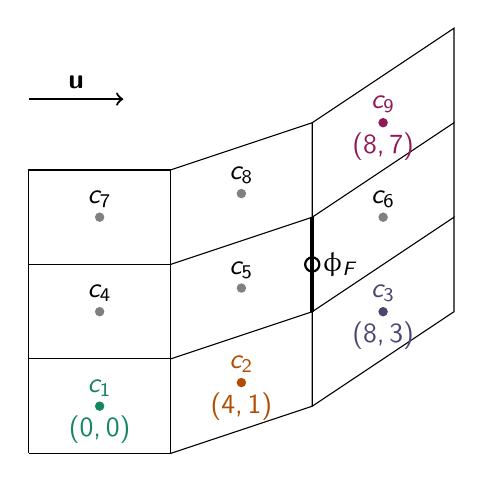
\begin{tikzpicture}[
  scale=0.6,
  cpnt/.style={fill=gray},
  font=\sffamily\sansmath
]
\draw [thick, ->] (0,7.5) -- (2,7.5) node [midway, anchor=south] {$\mathbf{u}$};

\draw (0,0) -- (3,0) -- (3,2) -- (0,2) -- (0,0);
\draw (0,2) -- (3,2) -- (3,4) -- (0,4) -- (0,2);
\draw (0,4) -- (3,4) -- (3,6) -- (0,6) -- (0,4);

\draw (3,0) -- (6,1) -- (6,3) -- (3,2);
\draw (6,3) -- (6,5) -- (3,4);
\draw (6,5) -- (6,7) -- (3,6);

\draw (6,1) -- (9,3) -- (9,5) -- (6,3);
\draw (9,5) -- (9,7) -- (6,5);
\draw (9,7) -- (9,9) -- (6,7);

\draw [ultra thick] (6,3) -- (6,5);
\draw [thick] (6,4) circle [radius=0.15] node [anchor=west] {$\phi_F$};

\path [cpnt,color={rgb:red,27;green,158;blue,119}] (1.5,1) circle [radius=0.1] node [anchor=south] {$c_1$} node [anchor=north] {$(0,0)$};
\path [cpnt] (1.5,3) circle [radius=0.1] node [anchor=south] {$c_4$};
\path [cpnt] (1.5,5) circle [radius=0.1] node [anchor=south] {$c_7$};

\path [cpnt,color={rgb:red,217;green,95;blue,2}] (4.5,1.5) circle [radius=0.1] node [anchor=south] {$c_2$} node [anchor=north] {$(4,1)$};
\path [cpnt] (4.5,3.5) circle [radius=0.1] node [anchor=south] {$c_5$};
\path [cpnt] (4.5,5.5) circle [radius=0.1] node [anchor=south] {$c_8$};

\path [cpnt,color={rgb:red,117;green,112;blue,179}] (7.5,3) circle [radius=0.1] node [anchor=south] {$c_3$} node [anchor=north] {$(8,3)$};
\path [cpnt] (7.5,5) circle [radius=0.1] node [anchor=south] {$c_6$};
\path [cpnt,color={rgb:red,231;green,41;blue,138}] (7.5,7) circle [radius=0.1] node [anchor=south] {$c_9$} node [anchor=north] {$(8,7)$};

\end{tikzpicture}
\end{document}
